\section*{Aufgabe 1a)}
In der ersten Teilaufgabe war zu zeigen, dass die gegebene Relation
$$C \equiv i(\hat{p} \hat{x} - \hat{x}\hat{p}) = 1$$ für beliebige, exakte Matrizen
nicht exakt gilt. Dafür wird die Spur der Operatoren in Matrixdarstellung
untersucht, für die diese Relation auch gelten muss, da es sich bei beiden Ausdrücken
um Diagonale Matrizen handelt. 
\begin{eqnarray}
Tr(\hat{p} \hat{x} - \hat{x}\hat{p}) &=& Tr(1) = N\\
&=& Tr(\hat{p} \hat{x}) - Tr(\hat{x}\hat{p})
\end{eqnarray}
Da für beliebige Matrizen $A,B$ gilt: $$Tr(A\cdot B) = Tr(B\cdot A)$$ ist der
obige Ausdruck null:
\begin{eqnarray}
Tr(\hat{p} \hat{x} - \hat{x}\hat{p}) &=& 0 \neq N
\end{eqnarray}
Da die Spuren des Orts-Impuls-Kommutators und der Einheitsmatrix nicht gleich sind,
ist auch die gegebene Relation selbst nicht exakt erfüllt.

\section*{Aufgabe 1b)}
In der Vorlesung wurde ein Ausdruck für $δ_{ij}$ über eine Fouriertransformation
gegeben: $$δ_{ij} = \frac{1}{N}\sum_p\exp(ip(x_k-x_l)).$$ 

Eine Wellenfunktion, die man sich aus Einträgen dieser Matrix zusammengesetzt
vorstellen kann, lässt sich demnach wie folgt über eine Fouriertransformation
darstellen:
\begin{eqnarray}
Ψ_k &=& \sum_l δ_{kl} = \frac{1}{L}\sum_p\tilde{Ψ}_p e^{ipx_k}\\
\tilde{Ψ}_p &=& a\sum_l Ψ_l e^{ipx_l}\\
\end{eqnarray}
Nun kann untersucht werden, wie ein quantenmechanischer Impulsoperator in
Matrixdarstellung auf eine solche Wellenfunktion wirkt:
\begin{eqnarray}
\hat{p}_{kl}Ψ_l &=& \frac{\hbar}{i}\frac{∂}{∂x_k}Ψ_l = \frac{1}{L}\sum_{p} p e^{ipx_k}\tilde{Ψ}_{p,l}\\
&=& \frac{a}{L}\sum_p p e^{ip(x_k-x_l)}Ψ_l
\end{eqnarray}
Über einen Koeffizientenvergleich kann nun $\hat{p}_{kl}$ unter Ausnutzung von
$N = La$ identifiziert werden:
\begin{eqnarray}
\hat{p}_{kl} = \frac{1}{N}\sum_p p e^{ip(x_k-x_l)}
\end{eqnarray}
Wenn man schließlich noch verwendet, dass es sich bei $\hat{p}$ um einen symmetrischen
Operator handelt, lässt sich diese Formel noch weiter vereinfachen:
\begin{eqnarray}
\hat{p}_{kl} = \frac{2i}{N}\sum_{|p|} |p| e^{i|p|(x_k-x_l)}
\end{eqnarray}
Diese Formel wurde schließlich implementiert. Der Quellcode für die Funktion, 
die den $p$-Operator generiert, ist in \lref{fkt} dargestellt.
\lstinputlisting[label=lst:fkt,caption={ho\_fou.m}]{../code/ho_fou.m}

Diese Funktion wird wie in \lref{1a} aufgerufen:
\lstinputlisting[lastline=2,label=lst:1a,caption={steuerung.m}]{../code/steuerung.m}

\section*{Aufgabe 1c)}
Das resultierende $C$, wie es mit Hilfe der Rückgabewerte des Aufrufs is Aufgabe 1b)
aus den zurückgegebenen Werten von $x$ und $p$ berechnet werden kann, lässt sich,
wie in \lref{1c} gezeigt, plotten, woraus \fref{mesh_c} resultiert.

\lstinputlisting[firstline=5,lastline=16,label=lst:1c,caption={steuerung.m}]{../code/steuerung.m}

\begin{figure}[htb]
  \centering
  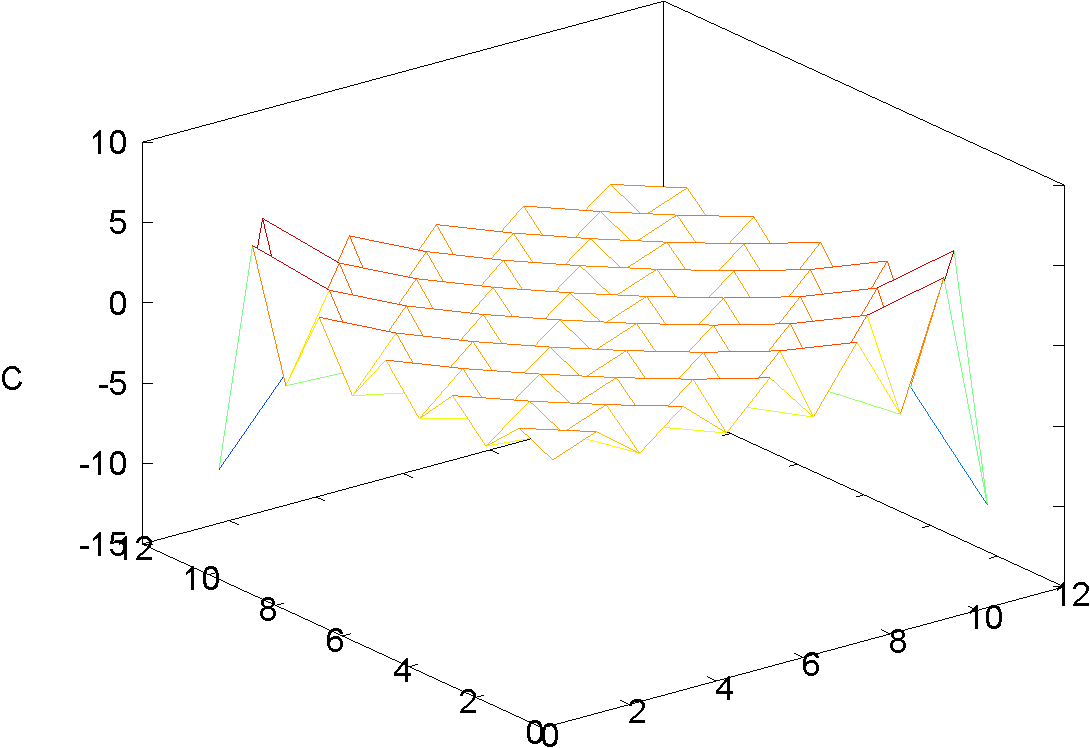
\includegraphics[width=0.8\columnwidth,keepaspectratio]{../tmp/mesh_c-crop}
  \caption{Mesh-Plot von $C$}
  \label{fig:mesh_c}
\end{figure}

Wie man erkennen kann, schwanken die Einträge in $C$ in der Größenordnung von 1, sodass
die Relation als näherungsweise erfüllt gelten kann.

\section*{Aufgabe 1d)}
Um zu überprüfen, ob die gegebene Relation erfüllt ist, wurden normierte Gaußfunktionen
erstellt und mit diesen wurden die gesuchten Skalarprodukte berechnet. 

\section*{Aufgabe 1e)}